% % % --------------------------------------------------------------------------------------
% % % ARPC Memo Template
% % % --------------------------------------------------------------------------------------

\documentclass{theme/arpc-memo}

% % % --------------------------------------------------------------------------------------
% % % Document Metadata (EDIT)
% % % --------------------------------------------------------------------------------------

\Authors{Shawn Arita, Matthew Gammans, Khashi Ghorbani, James Keeler}

\Title{ARPC Memo}

\Subtitle{TITLE}

\School{Agricultural Risk Policy Center, North Dakota State University}

%\AtBeginDocument{\renewcommand{\today}{October 24, 2025}}  % In case you want a different issuing date than \today

% % % --------------------------------------------------------------------------------------
% % % Main Document
% % % --------------------------------------------------------------------------------------

\begin{document}

% % % --------------------------------------------------------------------------------------
% % % Front Matter
% % % --------------------------------------------------------------------------------------

\RaggedRight

\AddToShipoutPictureBG{%
  \AtPageLowerLeft{
\includegraphics[width=\paperwidth,height=\paperheight]{theme/background/main.pdf}}%
}

\AddToShipoutPictureBG*{%
  \begin{tikzpicture}[remember picture,overlay]
    \clip (current page.south west) rectangle (current page.north east);
    \node[anchor=south west, xshift=-1.3mm, yshift=-1.3mm]
      at (current page.south west)
      {
\includegraphics[width=\paperwidth]{theme/background/front.pdf}};
  \end{tikzpicture}%
}

\vspace*{-2.5cm}\hspace*{-0.5cm}\noindent
\includegraphics[width=0.57\linewidth]{theme/background/logo.pdf}

\vspace*{0.75cm}

{\noindent\fontsize{20}{20}\selectfont{\color{ndsu}\centering\GetSubtitle\par}}

\vspace{0.5cm}

{\noindent\fontsize{13}{13}\selectfont{\bfseries\color{ndsu}\centering\GetSchool\par}}
\vspace{0.25cm}

{\noindent\fontsize{11}{11}\selectfont{\color{ndsu}\centering\today\par}}
\vspace*{0.25cm}

{\noindent\fontsize{13}{13}\selectfont{\bfseries \color{ndsu}\centering\GetTitle\par}

\vspace{0.25cm}

{\noindent\fontsize{13}{13}\selectfont{\color{red}\centering{FOR INTERNAL USE}\par}}

\noindent\hspace*{-\oddsidemargin}\hspace*{-1in}{\color{ndsu}\rule{\paperwidth}{2pt}}\par
\vspace*{-0.4cm}
{\noindent\fontsize{11}{11}\selectfont{{\color{ndsu} \bfseries Notice:}~\color{black} This memorandum is provided for internal awareness, coordination, and discussion, and the content may be refined as new data or feedback becomes available. Please keep circulation within the named recipients; please do not quote, post, or distribute externally without approval.}}}\par
\vspace*{-0.6cm}
\noindent\hspace*{-\oddsidemargin}\hspace*{-1in}{\color{ndsu}\rule{\paperwidth}{2pt}}\par
\vspace*{-1cm}


% % % --------------------------------------------------------------------------------------
% % % Main (EDIT)
% % % --------------------------------------------------------------------------------------

\section{Key Insights} % fit on one page

\begin{itemize}

\item {\textbf{\color{ndsu} Bla 1 is cool!}} Cool is bla 1.

\item  {\textbf{\color{ndsu} Bla 2 is cool!}} Cool is bla 2.

\item  {\textbf{\color{ndsu} Bla 3 is cool!}} Cool is bla 3.

\end{itemize}

\clearpage

\section{Background}

\lipsum[1-2]

\autoref{tab:trade_summary} summarizes the changes. \lipsum[1]  For this work, we cited \citet{Anderson2003} and the broader literature \citep[e.g.,][]{Yotov2016, Arita2025, Kim2025}.

\begin{table}[htpb!] % [htpb!] for float
\centering
\begin{threeparttable}
\captionsetup{justification=raggedright,singlelinecheck=true}
\caption{Summary of U.S. Agricultural Trade Indicators, 2018–2025.}
\label{tab:trade_summary}
\rowcolors{2}{lightgray}{white} % alternating row color
\small

% % % CHANGE THIS PART

\begin{tabular}{L{4.2cm} C{2.5cm} C{2.2cm} C{2.2cm} C{3.0cm}}
\toprule
\rowcolor{ndsu}
{\color{white}\bfseries Commodity} &
{\color{white}\bfseries 2018--2020 Avg.} &
{\color{white}\bfseries 2021} &
{\color{white}\bfseries 2022} &
{\color{white}\bfseries 2023--2025 (Proj.)} \\
\midrule
Corn Exports (MMT) & 55.3 & 61.8 & 53.1 & 50.0 \\
Soybean Exports (MMT) & 44.1 & 58.7 & 54.9 & 56.5 \\
Wheat Exports (MMT) & 26.2 & 22.7 & 20.1 & 19.8 \\
Beef Exports (Billion \$) & 8.4 & 10.7 & 11.3 & 12.1 \\
Pork Exports (Billion \$) & 6.5 & 7.8 & 7.4 & 7.2 \\
\midrule
\textbf{Total Ag Exports (Billion \$)} & \textbf{145.2} & \textbf{177.0} & \textbf{192.8} & \textbf{195.4} \\
\bottomrule
\end{tabular}

% % % % 

\vspace{1.5pt}
\begin{tablenotes}[flushleft]
\footnotesize
\setlength{\leftmargin}{0pt}      % remove item indentation
\setlength{\labelsep}{0pt}        % no gap before item text
\setlength{\itemsep}{4pt}         % vertical space between items
\setlength{\parsep}{0pt}          % no extra paragraph space
\setlength{\parindent}{0pt}       % no paragraph indent
\item\textit{Note:} Data represent calendar year exports. Projections for 2023–2025 are based on USDA baseline estimates. Data represent calendar year exports. Projections for 2023–2025 are based on USDA baseline estimates.\par
\item\textit{Source:} U.S. Department of Agriculture, Foreign Agricultural Service.
\end{tablenotes}
\end{threeparttable}
\end{table}

\subsection{Analysis of the Temporary Grain Storage Support Program}

The summary is provided in \autoref{fig:ag_exports}. \lipsum[1][1-28]

% \begin{figure}[h!] % [H] for no float
\captionsetup{justification=raggedright,singlelinecheck=true}
\caption{Trends in U.S. Agricultural Exports, 2018–2025.}
\label{fig:ag_exports}
\begin{threeparttable}
\centering

% --- chart ---
\begin{tikzpicture}
\begin{axis}[
  width=0.85\textwidth,
  height=8cm,
  ymin=0, ymax=150,
  ytick={0,25,50,75,100,125,150},
  yticklabels={0,25,50,75,100,125,150},  
  xlabel={Year},
  ylabel={Index (2018 = 100)},
  xtick=data,
  xticklabels={2018,2019,2020,2021,2022,2023,2024,2025},
  legend cell align={left}
]
  % Actual
  \addplot+[mark=*,
    mark options={fill=ndsu, draw=ndsu},
    color=ndsu, thick
  ] coordinates {(1,100) (2,103) (3,98) (4,107) (5,112) (6,115) (7,118) (8,121)};
  \addlegendentry{Actual Exports}

  % Projected
  \addplot+[mark=square*,
    mark options={fill=ndsuGold, draw=ndsuGold!100!black},
    color=ndsuGold!100!black, thick
  ] coordinates {(1,100) (2,102) (3,104) (4,108) (5,113) (6,118) (7,122) (8,126)};
  \addlegendentry{Projected Exports}
\end{axis}
\end{tikzpicture}

% --- notes/source, aligned to figure width ---
\vspace{3pt}
\begin{tablenotes}[flushleft]
\footnotesize
\setlength{\leftmargin}{0pt}      % remove item indentation
\setlength{\labelsep}{0pt}        % no gap before item text
\setlength{\itemsep}{4pt}         % vertical space between items
\setlength{\parsep}{0pt}          % no extra paragraph space
\setlength{\parindent}{0pt}       % no paragraph indent
\item \textit{Note:} Index values are normalized to 2018 = 100. Solid line indicates observed exports; dashed line shows projected growth. Solid line indicates observed exports; dashed line shows projected growth.
\item \textit{Source:} U.S. Department of Agriculture, Foreign Agricultural Service; ARPC analysis.
\end{tablenotes}

\end{threeparttable}
\end{figure}

\lipsum[1-3][1-28]

% \begin{figure}[t!] % [H] for no float
\captionsetup{justification=raggedright,singlelinecheck=true}
\caption{Brazil--U.S. soybean landed price with tariff in China differential by week and U.S. weekly net export sales to China.}
\label{fig:price_spread}
\begin{threeparttable}
% --- chart ---
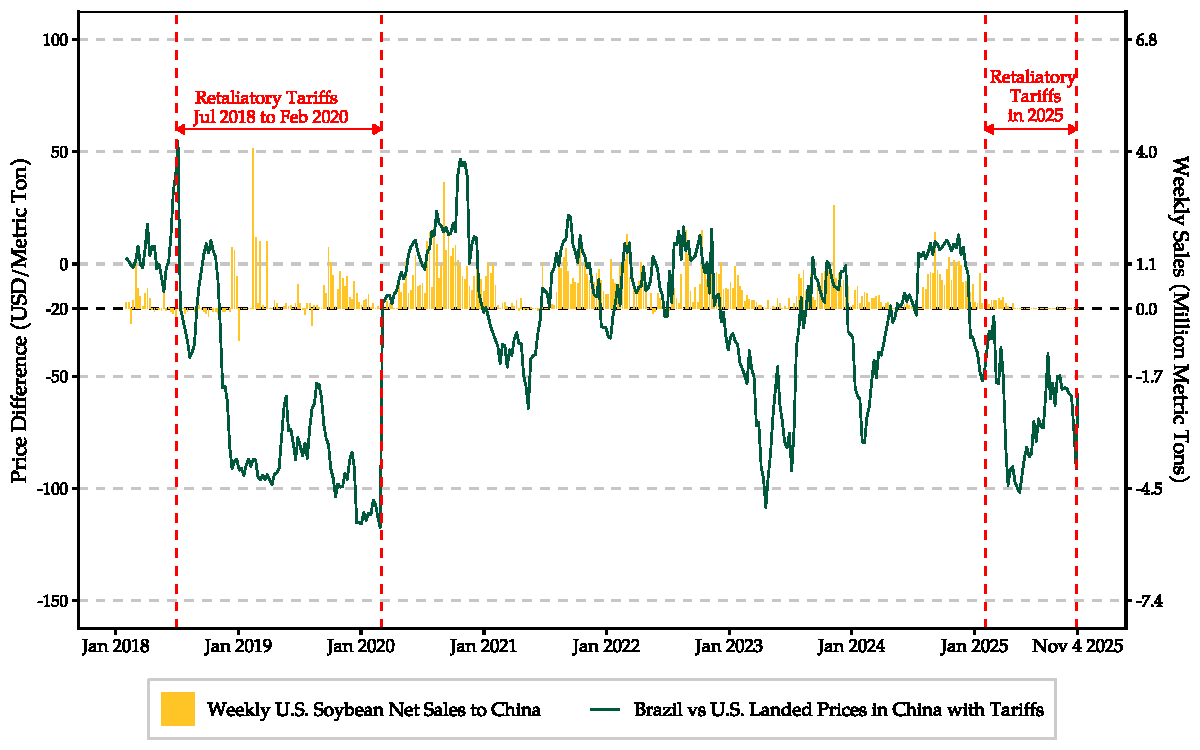
\includegraphics[width=0.95\linewidth]{visuals/figure2.pdf}
% --- notes/source, aligned to figure width ---
\vspace{3pt}
\begin{tablenotes}[flushleft]
\footnotesize
\setlength{\leftmargin}{0pt}      % remove item indentation
\setlength{\labelsep}{0pt}        % no gap before item text
\setlength{\itemsep}{4pt}         % vertical space between items
\setlength{\parsep}{0pt}          % no extra paragraph space
\setlength{\parindent}{0pt}       % no paragraph indent
\item \textit{Note:} Landed price in China includes shipping and insurance costs with tariffs (both MFN and retaliatory). The retaliatory tariff spike in April 2025 is not captured for presentation purposes.
\item \textit{Source:} DSU using data from Fastmarkets and USDA FAS Export Sales.
\end{tablenotes}

\end{threeparttable}
\end{figure}

\section{Conclusion}

\lipsum[1-3][1-28]

% % % --------------------------------------------------------------------------------------
% % % References
% % % --------------------------------------------------------------------------------------

\clearpage\printbibliography[title={References}]

% % % --------------------------------------------------------------------------------------
% % % Disclaimer and Back End
% % % --------------------------------------------------------------------------------------

\clearpage
\ClearShipoutPicture
\AddToShipoutPictureBG*{
\includegraphics{theme/background/back.pdf}}

\pagestyle{empty}
\begin{adjustwidth}{0pt}{0.44\textwidth}
\vspace*{-1.25cm}
{\color{ndsu}\crimsonfont\bfseries\fontsize{14}{17}\selectfont Disclaimer\par}
\vspace{0.6\baselineskip}
{\color{ndsu}\fontsize{11}{14}\selectfont
\noindent
\copyright~\the\year\ Agricultural Risk Policy Center at North Dakota State University. All rights reserved.\par}
\vspace{0.8\baselineskip}

\fontsize{11}{14}\selectfont
This publication is intended to contribute to ongoing discussions on agricultural policy and risk management. The analysis, findings, and conclusions represent the interpretation of the authors and do not necessarily reflect the views of North Dakota State University or any affiliated institution. The authors are solely responsible for any errors or omissions. Users of this publication are encouraged to consult additional data sources and expert perspectives when making policy, legal, or business decisions.\par
\end{adjustwidth}
\vspace{1.5cm}
\newcommand{\bigicon}[1]{{\color{ndsu}\raisebox{-0.1em}{\Large #1}}}
\begin{adjustwidth}{0pt}{0.2\textwidth}
\vspace{1em}
{\color{ndsu}\crimsonfont\bfseries\fontsize{14}{17}\selectfont Contact Us\par}
\vspace{1em}
\bigicon{\faEnvelope}\hspace{0.8em}\href{mailto:arpc@ndsu.edu}{arpc@ndsu.edu}\par
\vspace{0.3\baselineskip}
\bigicon{\faGlobe}\hspace{0.8em}\href{https://www.ndsu.edu/agriculture/arpc}{www.ndsu.edu/agriculture/arpc}\par
\vspace{0.3\baselineskip}
\bigicon{\faMapMarker*}\hspace{0.8em}
\href{https://www.google.com/maps?q=Richard+H.+Barry+Hall,+811+2nd+Ave+N,+Fargo,+ND+58102}{
Richard H. Barry Hall 400, Fargo, ND}\par
\vspace{0.3\baselineskip}
\bigicon{\faLinkedin}\hspace{0.8em}\href{https://www.linkedin.com/company/ndsu-agricultural-risk-policy-center}{
https://www.linkedin.com/company/ndsu-agricultural-risk-policy-center}\par
\vspace{1em}
\end{adjustwidth}
\vfill
\begin{tikzpicture}[remember picture,overlay]
\node[anchor=south, yshift=0.2cm] 
at (current page.south)
{
\includegraphics[width=0.57\linewidth]{theme/background/logo.pdf}};
\end{tikzpicture}

% % % --------------------------------------------------------------------------------------
% % % Closure
% % % --------------------------------------------------------------------------------------

\end{document}